% Options for packages loaded elsewhere
\PassOptionsToPackage{unicode}{hyperref}
\PassOptionsToPackage{hyphens}{url}
\PassOptionsToPackage{dvipsnames,svgnames*,x11names*}{xcolor}
%
\documentclass[
  12pt,
  portuguese,
]{article}
\usepackage{lmodern}
\usepackage{setspace}
\usepackage{amsmath}
\usepackage{ifxetex,ifluatex}
\ifnum 0\ifxetex 1\fi\ifluatex 1\fi=0 % if pdftex
  \usepackage[T1]{fontenc}
  \usepackage[utf8]{inputenc}
  \usepackage{textcomp} % provide euro and other symbols
  \usepackage{amssymb}
\else % if luatex or xetex
  \usepackage{unicode-math}
  \defaultfontfeatures{Scale=MatchLowercase}
  \defaultfontfeatures[\rmfamily]{Ligatures=TeX,Scale=1}
\fi
% Use upquote if available, for straight quotes in verbatim environments
\IfFileExists{upquote.sty}{\usepackage{upquote}}{}
\IfFileExists{microtype.sty}{% use microtype if available
  \usepackage[]{microtype}
  \UseMicrotypeSet[protrusion]{basicmath} % disable protrusion for tt fonts
}{}
\usepackage{xcolor}
\IfFileExists{xurl.sty}{\usepackage{xurl}}{} % add URL line breaks if available
\IfFileExists{bookmark.sty}{\usepackage{bookmark}}{\usepackage{hyperref}}
\hypersetup{
  pdftitle={Ensino remoto emergencial durante a COVID-19: Percepções de estudantes de Ciência da Computação da UFCG},
  pdflang={pt},
  colorlinks=true,
  linkcolor=blue,
  filecolor=Maroon,
  citecolor=Blue,
  urlcolor=Blue,
  pdfcreator={LaTeX via pandoc}}
\urlstyle{same} % disable monospaced font for URLs
\usepackage[margin=1in]{geometry}
\usepackage{longtable,booktabs}
\usepackage{calc} % for calculating minipage widths
% Correct order of tables after \paragraph or \subparagraph
\usepackage{etoolbox}
\makeatletter
\patchcmd\longtable{\par}{\if@noskipsec\mbox{}\fi\par}{}{}
\makeatother
% Allow footnotes in longtable head/foot
\IfFileExists{footnotehyper.sty}{\usepackage{footnotehyper}}{\usepackage{footnote}}
\makesavenoteenv{longtable}
\usepackage{graphicx}
\makeatletter
\def\maxwidth{\ifdim\Gin@nat@width>\linewidth\linewidth\else\Gin@nat@width\fi}
\def\maxheight{\ifdim\Gin@nat@height>\textheight\textheight\else\Gin@nat@height\fi}
\makeatother
% Scale images if necessary, so that they will not overflow the page
% margins by default, and it is still possible to overwrite the defaults
% using explicit options in \includegraphics[width, height, ...]{}
\setkeys{Gin}{width=\maxwidth,height=\maxheight,keepaspectratio}
% Set default figure placement to htbp
\makeatletter
\def\fps@figure{htbp}
\makeatother
\setlength{\emergencystretch}{3em} % prevent overfull lines
\providecommand{\tightlist}{%
  \setlength{\itemsep}{0pt}\setlength{\parskip}{0pt}}
\setcounter{secnumdepth}{5}
\usepackage{floatrow}
\floatsetup[figure]{capposition=top}
\usepackage{booktabs}
\usepackage{longtable}
\usepackage{array}
\usepackage{multirow}
\usepackage{wrapfig}
\usepackage{float}
\usepackage{colortbl}
\usepackage{pdflscape}
\usepackage{tabu}
\usepackage{threeparttable}
\usepackage{threeparttablex}
\usepackage[normalem]{ulem}
\usepackage{makecell}
\usepackage{xcolor}
\ifxetex
  % Load polyglossia as late as possible: uses bidi with RTL langages (e.g. Hebrew, Arabic)
  \usepackage{polyglossia}
  \setmainlanguage[]{portuguese}
\else
  \usepackage[shorthands=off,main=portuguese]{babel}
\fi
\ifluatex
  \usepackage{selnolig}  % disable illegal ligatures
\fi
\newlength{\cslhangindent}
\setlength{\cslhangindent}{1.5em}
\newlength{\csllabelwidth}
\setlength{\csllabelwidth}{3em}
\newenvironment{CSLReferences}[2] % #1 hanging-ident, #2 entry spacing
 {% don't indent paragraphs
  \setlength{\parindent}{0pt}
  % turn on hanging indent if param 1 is 1
  \ifodd #1 \everypar{\setlength{\hangindent}{\cslhangindent}}\ignorespaces\fi
  % set entry spacing
  \ifnum #2 > 0
  \setlength{\parskip}{#2\baselineskip}
  \fi
 }%
 {}
\usepackage{calc}
\newcommand{\CSLBlock}[1]{#1\hfill\break}
\newcommand{\CSLLeftMargin}[1]{\parbox[t]{\csllabelwidth}{#1}}
\newcommand{\CSLRightInline}[1]{\parbox[t]{\linewidth - \csllabelwidth}{#1}\break}
\newcommand{\CSLIndent}[1]{\hspace{\cslhangindent}#1}

\title{Ensino remoto emergencial durante a COVID-19: Percepções de
estudantes de Ciência da Computação da UFCG}
\author{}
\date{\vspace{-2.5em}19 de Setembro de 2020}

\begin{document}
\maketitle

\setstretch{1}
\begin{quote}
\textbf{Abstract}: \emph{The outbreak of the new coronavirus will likely
go down in history, not only for the implications it has brought to
global health, but also for the changes it has brought about in various
areas. Among these, education has undergone major transformations, and
emergency remote teaching emerged as a response to the pandemic, which
made it impossible to continue in-person classes. In this article, we
will analyze the perceptions of computer science students, from the
Federal University of Campina Grande (UFCG), about learning under the
new imposed conditions. We carried out a survey and, through an online
form, we collected responses from students from different periods of the
course, focusing on questions that would allow us to understand the
degree in which some difficulties affect them, as well as some positive
points, from the point of view of different classes of course subjects
(practical/laboratories, computer theory/general subjects and
mathematics/statistics). The results of this study suggest that, on the
negative side, the study environment appears as a great difficulty for
students during emergency remote teaching. On the positive side, the
flexibility, a characteristic of this type of teaching, appears as a
great advantage for students in the course and it is possible that there
is a slight improvement in the students' perceived learning.}
\end{quote}

\begin{quote}
\textbf{Keywords}: Emergency remote teaching, COVID-19, student
perceptions, learning, survey.
\end{quote}

\newpage

\begin{quote}
\textbf{Resumo}: \emph{O surto do novo coronavírus provavelmente ficará
marcado na história, não apenas pelas implicações que trouxe para a
saúde global, mas também pelas mudanças que provocou em várias áreas.
Dentre essas, a educação passou por grandes transformações, e o ensino
remoto emergencial surgiu como uma resposta à pandemia, que
impossibilitou o prosseguimento de aulas presenciais. Nesse artigo,
analisaremos as percepções de estudantes de ciência da computação, da
Universidade Federal de Campina Grande (UFCG), acerca da aprendizagem
nas novas condições impostas. Realizamos uma pesquisa survey e, através
de um formulário online, coletamos respostas de alunos de diversos
períodos do curso, focando em perguntas que nos permitissem entender o
grau de prejuízo de algumas dificuldades, bem como o grau de satisfação
com alguns pontos positivos do ensino remoto, a partir do ponto de vista
de diferentes classes de disciplinas do curso (práticas, teóricas de
computação/gerais e teóricas de matemática/estatística). Os resultados
desse estudo sugerem que, por um lado negativo, o ambiente de estudo
aparece como grande dificuldade para os estudantes durante o ensino
remoto emergencial. Analisando por um lado positivo, a flexibilização
dos horários, característica desse tipo de ensino, surge como grande
vantagem para os alunos do curso e é possível que haja uma leve melhora
no aprendizado percebido dos estudantes.}
\end{quote}

\begin{quote}
\textbf{Palavras-chave}: Ensino remoto emergencial, COVID-19, percepções
de estudantes, aprendizagem, survey.
\end{quote}

\setstretch{1.5}

\hypertarget{introduuxe7uxe3o}{%
\section{Introdução}\label{introduuxe7uxe3o}}

O surto do novo coronavírus em 2020 marcou o começo de uma mudança
drástica no cotidiano das pessoas e na dinâmica das instituições
públicas e privadas em todo o mundo, incluindo as de ensino superior. Em
11 de março de 2020, a Organização Mundial da Saúde (OMS) caracterizou a
COVID-19 como uma pandemia (\protect\hyperlink{ref-who}{GHEBREYESUS,
2020}), e daí por diante observou-se de perto e cotidianamente o avanço
do vírus, responsável por milhares de mortes não apenas no Brasil, mas
no mundo inteiro. Nesse contexto, torna-se inevitável falar sobre os
impactos nas instituições de ensino superior
(\protect\hyperlink{ref-compassionate}{GELLES et al., 2020};
\protect\hyperlink{ref-biopolitica}{JESUS PEREIRA; NARDUCHI; MIRANDA,
2020}), as quais foram obrigadas a migrar para regimes remotos de
aprendizado, para os quais a maioria não estava preparada.

E como muitas outras, a Universidade Federal de Campina Grande também
adotou esse regime como alternativa para a continuidade dos seus cursos.
Com isso, há pouco mais de um ano, os discentes da UFCG viram suas
rotinas mudarem profundamente, precisando adaptá-las ao novo sistema de
ensino. Nesse ponto, criam-se muitas expectativas para o desenrolar
dessa situação, vários questionamentos surgem frente a um desafio nunca
antes vivenciado. Dúvidas acerca do desempenho dos estudantes, bem como
pontos positivos e negativos do ensino remoto, que antes não era sequer
cogitado, passam agora a serem considerados
(\protect\hyperlink{ref-positives}{MUCCI-FERRIS; GRABSCH; BOBO, 2021}).
Dessa forma, destaca-se a importância do estudo realizado não apenas por
levantar as dificuldades dos estudantes em um novo sistema de ensino,
mas também por considerar os impactos positivos do mesmo, sendo até
mesmo possível, em uma próxima discussão, considerar a adaptação de
alguns deles para o ensino presencial.

Nesse artigo, vamos focar em compreender e analisar as percepções dos
estudantes de Ciência da Computação, especificamente do departamento da
UFCG, a respeito da aprendizagem durante o ensino remoto emergencial.
Através de uma survey, estudamos os graus de prejuízo trazidos por
algumas dificuldades comuns na literatura, como também procuramos
entender o grau de satisfação com alguns pontos positivos, consequências
do ensino remoto, também levantados em artigos recentes. Levamos em
consideração, ainda, diferentes classes de disciplinas no curso
(práticas/laboratórios, teóricas de computação/gerais e teóricas de
matemática/estatística), uma vez que, dificuldades de disciplinas
teóricas podem não ser as mesmas das disciplinas práticas.

Nossos resultados sugerem que, apesar dos estudantes de computação já
possuírem familiaridade com ferramentas online, certos aspectos do
ensino remoto, como os ambientes não produtivos de suas casas, ainda
representam um empecilho que os prejudica. Entretanto, observamos
considerável grau de satisfação acerca dos pontos positivos, aliado aos
seus aprendizados percebidos, os quais podem ter melhorado levemente em
relação ao ensino presencial. De forma geral, o restante deste artigo é
composto pelas seguintes seções complementares: Trabalhos relacionados,
materiais e métodos, resultados, discussão, conclusão e declarações
(conflitos de interesse e dados da pesquisa).

\hypertarget{trabalhos-relacionados}{%
\section{Trabalhos relacionados}\label{trabalhos-relacionados}}

A pandemia causada pela COVID-19 trouxe consigo vários desafios às
instituições de educação superior, todavia ela não foi a primeira crise
que ocasionou migração para um ensino remoto emergencial. Desastres
naturais, como terremotos
(\protect\hyperlink{ref-gomez2013lessons}{GÓMEZ, 2013}) e furacões
(\protect\hyperlink{ref-dicarlo2007survival}{DICARLO et al., 2007}),
protestos estudantis
(\protect\hyperlink{ref-czerniewicz2019online}{CZERNIEWICZ; TROTTER;
HAUPT, 2019}), guerras e conflitos
(\protect\hyperlink{ref-schweber2008determined}{SCHWEBER, 2008}) também
resultaram na adoção temporária desse regime. Nem tão pouco essa
pandemia foi a única, outro exemplo que ocasionou disrupções regionais
foi a provocada pela H1N1 (\protect\hyperlink{ref-van2010university}{VAN
et al., 2010}), com isso dito, o novo coronavírus afetou a vida de
praticamente todos em uma escala nunca antes vista e mudou a dinâmica de
países inteiros por mais de um ano e dá sinais que não irá parar tão
cedo (\protect\hyperlink{ref-timeline}{TAYLOR, 2020}).

Situações como as descritas, apesar de trágicas, foram acompanhadas de
pesquisas sobre a resposta da educação superior e sua transição para o
regime remoto. Isso inclui a rápida adaptação para o ensino online
(\protect\hyperlink{ref-mackey2012blended}{MACKEY et al., 2012}), a
importância de comunicação clara e transparente entre universidade e
estudantes (\protect\hyperlink{ref-gomez2013lessons}{GÓMEZ, 2013}),
discussões de equidade e ética
(\protect\hyperlink{ref-swartz2018care}{SWARTZ; GACHAGO; BELFORD,
2018}), análise de sentimento automatizado (e.g.~tweets)
(\protect\hyperlink{ref-duong2020ivory}{DUONG et al., 2020}) e análise
de repercussão em classes de alunos
(\protect\hyperlink{ref-compassionate}{GELLES et al., 2020};
\protect\hyperlink{ref-petillion2020student}{PETILLION; MCNEIL, 2020}).

Outro tema recorrente é o de saúde mental e física de estudantes e
instrutores (\protect\hyperlink{ref-cao2020psychological}{CAO et al.,
2020}), como também o impacto do regime remoto na experiência de
aprendizado. O que fez surgir pesquisas sobre as percepções dos
discentes em tempo de ensino remoto
(\protect\hyperlink{ref-toti2021}{TOTI; ALIPOUR, 2021}), as quais
analisaram aspectos como dificuldades e pontos positivos. A literatura
nos mostra que estudantes não confiam em suas habilidades de focar nos
trabalhos escolares em casa, onde outras distrações estão presentes,
dificultando a realização de trabalhos em grupo
(\protect\hyperlink{ref-zimmerman2016online}{ZIMMERMAN; KULIKOWICH,
2016}). Além disso, também são listados como problemas fatores como a
falta de infraestrutura \protect\hyperlink{ref-dhawan2020online}{DHAWAN}
(\protect\hyperlink{ref-dhawan2020online}{2020}), motivação e ritmo na
ausência de cronograma estruturado
(\protect\hyperlink{ref-fedynich2013teaching}{FEDYNICH, 2013}).

Também existem estudos que focam em alunos de Ciência da Computação,
Maltby e Whittle (\protect\hyperlink{ref-maltby2000learning}{MALTBY;
WHITTLE, 2000}) mostraram opiniões conflituosas de estudantes, enquanto
58\% dos entrevistados indicaram uma preferência por aulas face-a-face
em relação às online, acreditando terem mais valor educacional, outros
viram com bons olhos o fato das aulas estarem disponíveis online,
podendo ser acessadas facilmente e de forma flexível, e ao mesmo tempo
teve aqueles frustrados por problemas com conectividade e dificuldade em
perguntar questões aos instrutores.

Em um estudo mais recente por Toti e Alipour
(\protect\hyperlink{ref-toti2021}{TOTI; ALIPOUR, 2021}), foram
analisadas as percepções de alunos de Ciência da Computação na transição
de ensino presencial para o remoto na Universidade de Houston (Texas) e,
dentre outras coisas, apontou-se dificuldades como a de perguntar
questões em sala e interagir com os instrutores, e experiência
favoráveis aos alunos como a flexibilidade de poder acessar e estudar
materiais disponibilizados assincronamente e em seu ritmo. Também foi
citado que alguns professores tornaram seus planos de aula mais claros e
usaram de comunicação menos ambígua, o que também foi avaliado de forma
positiva.

Considerando todo o nosso conhecimento, a experiência de estudantes de
Ciência da Computação no Brasil, no contexto de avaliação de
dificuldades e pontos positivos pelos alunos, ainda não foi investigada
e beneficiaria a comunidade acadêmica. Neste trabalho, nosso objetivo é
justamente esse, compreender melhor em que grau as principais
dificuldades reportadas na literatura os prejudicam e quais
características mais os satisfazem no contexto remoto. Para isso,
analisamos um grupo de estudantes de um dos cursos de ciência da
computação mais bem avaliados no Brasil, ofertado pela Universidade
Federal de Campina Grande - UFCG.

\hypertarget{materiais-e-muxe9todos}{%
\section{Materiais e Métodos}\label{materiais-e-muxe9todos}}

Com o objetivo de entender melhor a percepção dos estudantes de Ciência
da Computação da UFCG acerca de dificuldades, pontos positivos e
aprendizado percebido durante o ensino remoto emergencial, realizamos um
questionário anônimo composto por 15 perguntas objetivas, abertas e com
escala, o qual foi distribuído na lista de emails do curso e as
respostas coletadas online. O convite para participar da pesquisa foi
enviado em 10 de agosto de 2021 e as respostas foram coletadas até 16 de
agosto.

A primeira seção do questionário teve o objetivo de coletar informações
pessoais sobre os alunos, incluindo idade, gênero, o período de ingresso
na universidade e qual classe(s) de disciplinas cursou ou está cursando
no ensino remoto emergencial. Já a segunda está relacionada às
dificuldades que os alunos enfrentaram até o momento no ensino remoto ao
cursarem disciplinas teóricas de matemática e/ou estatística (TM/E), de
computação e/ou optativas gerais (TC/OG) e em práticas e/ou laboratórios
(P/L). Com o objetivo de identificar qual problema mais prejudica os
estudantes e quais disciplinas são mais afetadas. Dentre as dificuldades
foram enumerados problemas técnicos (PT), problemas de comunicação com o
professor (CP), problema de gerenciamento de tempo (GT), falta de
contato pessoal com o professor (FC) e distrações por não estar em um
ambiente não produtivo (ANP). Para medir o prejuízo associado às
dificuldades foi utilizada escala Likert de 5 pontos, que varia de ``Não
fui prejudicado'' a ``Fui muito prejudicado''.

Na terceira seção de perguntas são coletadas informações sobre possíveis
pontos positivos ocasionados pelo ensino remoto e o quanto ajudaram os
alunos. Dentre esses pontos, estão os horários flexíveis de estudo (HF),
já que muitas disciplinas disponibilizam aulas gravadas, além de não
cobrarem faltas. Estrutura mais clara das disciplinas (EC), e
aprendizado no ritmo próprio do aluno (RP) foram outros pontos
questionados nesta seção. A escala Likert de 5 pontos também foi
utilizada nessa seção variando de ``Não me ajudaram'' a ``Me ajudaram
bastante''.

Na quarta e última seção, o aluno é questionado sobre o quanto seu
aprendizado foi afetado no ensino remoto, usando mais uma vez a escala
Likert que varia de ``Eu aprendi bem menos'' a ``Eu aprendi bem mais''.
E de forma opcional é interrogado sobre quais dificuldades e quais
pontos positivos que não foram citados na seções anteriores tiveram que
enfrentar.

\hypertarget{resultados}{%
\section{Resultados}\label{resultados}}

A pesquisa contou com 67 respostas e as características dos
participantes podem ser sumarizadas da seguinte forma:

\begin{itemize}
\tightlist
\item
  Idade: Média de 21.87 anos (desvio padrão: 2.77), com 94\% dos
  participantes entre 18-25 anos e o restante (6\%) de 28-34 anos.
\item
  Gênero: 80.6\% (n = 54) se declararam do masculino e 19.4\% (n = 13)
  feminino.
\item
  Período de ingresso na faculdade: As maiores proporções foram de
  23.9\% no primeiro semestre de 2018 (2018.1), 17.9\% no segundo
  semestre de 2017 (2017.2) e 10.4\% no segundo semestre de 2020
  (2020.2). O restante obteve menos de 9\% cada.
\item
  Classe de disciplinas cursadas ou cursando: 97.01\% indicaram teóricas
  de computação e/ou optativas gerais (TC/OG), 80.6\% teóricas de
  matemática e/ou estatística (TM/E) e 70.15\% práticas e/ou
  laboratórios (P/L).
\end{itemize}

A seguir, apresentamos estatísticas e distribuições das questões que se
utilizaram de escala Likert para quantificar a percepção dos estudantes.
Com respeito às dificuldades e pontos positivos nas 3 classes de
disciplinas, consideramos apenas as respostas daqueles que cursaram ou
estão cursando alguma matéria incluída na respectiva classe.

A primeira parte da pesquisa avaliou o prejuízo percebido, o qual os
estudantes associaram a 5 dificuldades encontradas na literatura, por
classe de disciplinas (TC/OG, TM/E e P/L). Já a escala variou de ``não
fui prejudicado'' à ``fui muito prejudicado''. A distribuição das
respostas pode ser encontrada na tabela 1, enquanto as médias de
prejuízo e seus intervalos de confiança estão na figura 1. Para a
técnica de estimativa desses intervalos, usamos bootstrapping com 4000
reamostragens e correção de viés
(\protect\hyperlink{ref-efron1992bootstrap}{EFRON, 1992}).

Enquanto a segunda parte da pesquisa tratou da ajuda percebida que os
estudantes associam a 3 pontos positivos, também pelas mesmas classes de
disciplinas. A escala variou de ``não me ajudaram'' à ``fui ajudado
bastante''. As estatísticas e distribuições igualmente se encontram na
tabela 1 e figura 2.

A terceira parte tanto coletou dificuldades e pontos positivos que os
estudantes observaram, que não foram citadas na pesquisa, como também
questionou o grau de aprendizado percebido por eles em meio ao ensino
remoto emergencial de 1-10. A escala variou de ``aprendi bem menos'' à
``aprendi bem mais''. A média geral foi de 5.6 (n = 67, IC 95\% =
{[}5.01, 6.16{]}), enquanto que analisando só para os de gênero
masculino foi de 5.57 (n = 54, desvio padrão = 2.28, IC 95\% = {[}4.98,
6.19{]}) e feminino foi de 5.69 (n = 13, desvio padrão = 2.95, IC 95\% =
{[}4.23, 7.23{]}).

\newpage

\begingroup\fontsize{10}{12}\selectfont

\begin{ThreePartTable}
\begin{TableNotes}
\item \textit{Note: } 
\item MP Muito Pouco, P Pouco, N Neutro, R Razoável, M Muito
\item Nos pontos positivos diz respeito a satisfação e nas dificuldades ao grau de prejuízo
\end{TableNotes}
\begin{longtable}[t]{l|l|l|l|l|l|l|r}
\caption{\label{tab:likertdifficulties}Graus de dificuldade e satisfação com pontos positivos}\\
\hline
Aspecto & Disciplina & 1-MP & 2-P & 3-N & 4-R & 5-M & Média\\
\hline
\multicolumn{8}{l}{\textbf{Experiências negativas}}\\
\hline
\hspace{1em} & TC/OG & 10.8 \% & 16.9 \% & 13.8 \% & 29.2 \% & 29.2 \% & 3.49\\
\cline{2-8}\nopagebreak
\hspace{1em} & TM/E & 16.7 \% & 13 \% & 13 \% & 29.6 \% & 27.8 \% & 3.39\\
\cline{2-8}\nopagebreak
\hspace{1em}\multirow{-3}{*}{\raggedright\arraybackslash Ambiente não produtivo} & P/L & 14.9 \% & 14.9 \% & 14.9 \% & 31.9 \% & 23.4 \% & 3.34\\
\cline{1-8}\pagebreak[0]
\hspace{1em} & TC/OG & 27.7 \% & 30.8 \% & 20 \% & 16.9 \% & 4.6 \% & 2.40\\
\cline{2-8}\nopagebreak
\hspace{1em} & TM/E & 25.9 \% & 31.5 \% & 24.1 \% & 11.1 \% & 7.4 \% & 2.43\\
\cline{2-8}\nopagebreak
\hspace{1em}\multirow{-3}{*}{\raggedright\arraybackslash Comunicação prejudicada} & P/L & 29.8 \% & 29.8 \% & 12.8 \% & 17 \% & 10.6 \% & 2.49\\
\cline{1-8}\pagebreak[0]
\hspace{1em} & TC/OG & 16.9 \% & 18.5 \% & 29.2 \% & 18.5 \% & 16.9 \% & 3.00\\
\cline{2-8}\nopagebreak
\hspace{1em} & TM/E & 24.1 \% & 20.4 \% & 20.4 \% & 16.7 \% & 18.5 \% & 2.85\\
\cline{2-8}\nopagebreak
\hspace{1em}\multirow{-3}{*}{\raggedright\arraybackslash Falta de contato} & P/L & 25.5 \% & 12.8 \% & 21.3 \% & 19.1 \% & 21.3 \% & 2.98\\
\cline{1-8}\pagebreak[0]
\hspace{1em} & TC/OG & 23.1 \% & 24.6 \% & 16.9 \% & 23.1 \% & 12.3 \% & 2.77\\
\cline{2-8}\nopagebreak
\hspace{1em} & TM/E & 31.5 \% & 14.8 \% & 13 \% & 25.9 \% & 14.8 \% & 2.78\\
\cline{2-8}\nopagebreak
\hspace{1em}\multirow{-3}{*}{\raggedright\arraybackslash Prob. de Gerenciamento de tempo} & P/L & 23.4 \% & 23.4 \% & 27.7 \% & 12.8 \% & 12.8 \% & 2.68\\
\cline{1-8}\pagebreak[0]
\hspace{1em} & TC/OG & 55.4 \% & 18.5 \% & 18.5 \% & 6.2 \% & 1.5 \% & 1.80\\
\cline{2-8}\nopagebreak
\hspace{1em} & TM/E & 59.3 \% & 20.4 \% & 9.3 \% & 11.1 \% & 0 \% & 1.72\\
\cline{2-8}\nopagebreak
\hspace{1em}\multirow{-3}{*}{\raggedright\arraybackslash Problemas técnicos} & P/L & 53.2 \% & 17 \% & 10.6 \% & 12.8 \% & 6.4 \% & 2.02\\
\cline{1-8}\pagebreak[0]
\multicolumn{8}{l}{\textbf{Experiências positivas}}\\
\hline
\hspace{1em} & TC/OG & 6.2 \% & 12.3 \% & 21.5 \% & 24.6 \% & 35.4 \% & 3.71\\
\cline{2-8}\nopagebreak
\hspace{1em} & TM/E & 3.7 \% & 16.7 \% & 18.5 \% & 24.1 \% & 37 \% & 3.74\\
\cline{2-8}\nopagebreak
\hspace{1em}\multirow{-3}{*}{\raggedright\arraybackslash Estrutura clara} & P/L & 6.4 \% & 17 \% & 17 \% & 27.7 \% & 31.9 \% & 3.62\\
\cline{1-8}\pagebreak[0]
\hspace{1em} & TC/OG & 3.1 \% & 4.6 \% & 10.8 \% & 21.5 \% & 60 \% & 4.31\\
\cline{2-8}\nopagebreak
\hspace{1em} & TM/E & 1.9 \% & 7.4 \% & 7.4 \% & 22.2 \% & 61.1 \% & 4.33\\
\cline{2-8}\nopagebreak
\hspace{1em}\multirow{-3}{*}{\raggedright\arraybackslash Horário Flexível} & P/L & 4.3 \% & 8.5 \% & 6.4 \% & 23.4 \% & 57.4 \% & 4.21\\
\cline{1-8}\pagebreak[0]
\hspace{1em} & TC/OG & 0 \% & 15.4 \% & 26.2 \% & 23.1 \% & 35.4 \% & 3.78\\
\cline{2-8}\nopagebreak
\hspace{1em} & TM/E & 5.6 \% & 16.7 \% & 16.7 \% & 25.9 \% & 35.2 \% & 3.69\\
\cline{2-8}\nopagebreak
\hspace{1em}\multirow{-3}{*}{\raggedright\arraybackslash Ritmo próprio} & P/L & 2.1 \% & 17 \% & 25.5 \% & 21.3 \% & 34 \% & 3.68\\
\hline
\insertTableNotes
\end{longtable}
\end{ThreePartTable}
\endgroup{}

\begin{figure}
\centering
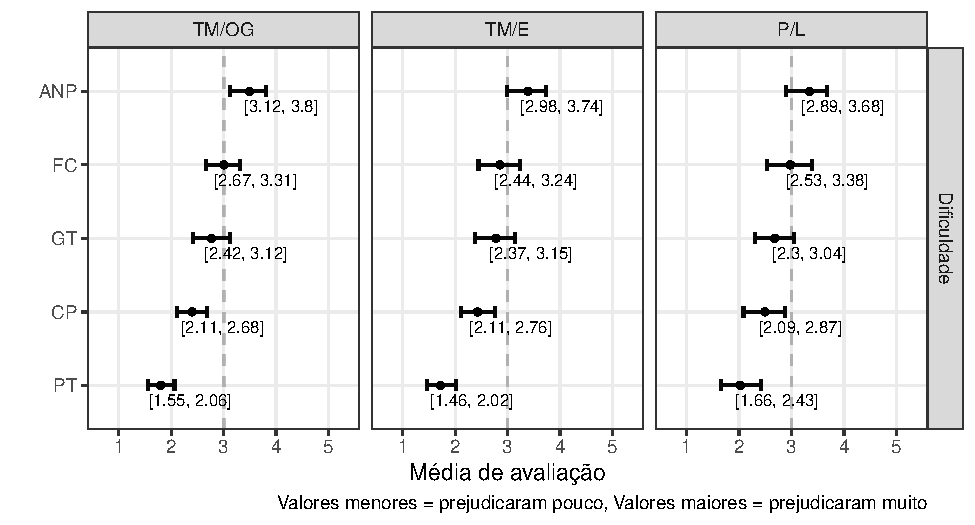
\includegraphics{paper_files/figure-latex/dificuldades-1.pdf}
\caption{\label{fig:fig1} Graus de prejuízo das dificuldades}
\end{figure}

\begin{figure}
\centering
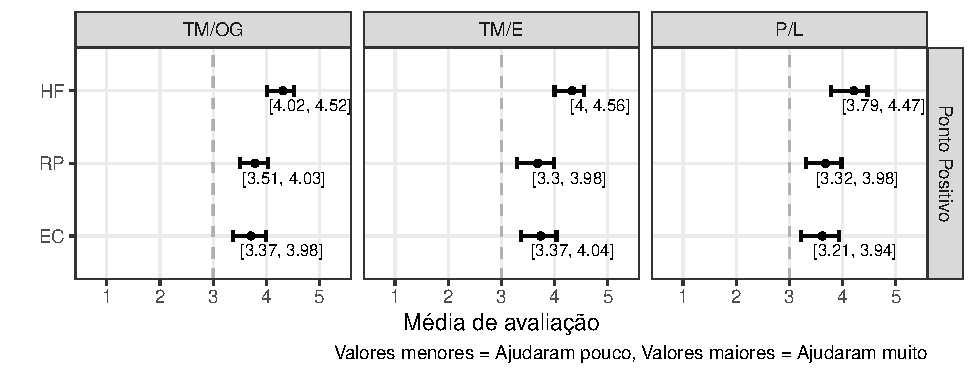
\includegraphics{paper_files/figure-latex/pontos_positivos-1.pdf}
\caption{\label{fig:fig2} Graus de satisfação com os pontos positivos}
\end{figure}

\hypertarget{anuxe1lise-das-respostas-uxe0s-questuxf5es-abertas}{%
\subsection{Análise das respostas às questões
abertas}\label{anuxe1lise-das-respostas-uxe0s-questuxf5es-abertas}}

O formulário conteve duas questões abertas opcionais (1) quais
dificuldades (não citadas anteriormente) os impactaram negativamente e
(2) quais pontos (não citados anteriormente) os impactaram
positivamente. Identificamos e categorizamos cada resposta dos alunos. A
tabela 2 mostra as principais categorias das respostas e as suas
frequências. No restante da seção sumarizamos as experiências positivas
e as dificuldades causadas pelo ensino remoto emergencial relatadas.

\setstretch{0}

\begin{longtable}[]{@{}lll@{}}
\caption{Frequência das categorias nas questões abertas}\tabularnewline
\toprule
\begin{minipage}[b]{(\columnwidth - 2\tabcolsep) * \real{0.42}}\raggedright
Categoria\strut
\end{minipage} &
\begin{minipage}[b]{(\columnwidth - 2\tabcolsep) * \real{0.19}}\raggedright
Frequência\strut
\end{minipage} &
\begin{minipage}[b]{(\columnwidth - 2\tabcolsep) * \real{0.21}}\raggedright
Tipo\strut
\end{minipage}\tabularnewline
\midrule
\endfirsthead
\toprule
\begin{minipage}[b]{(\columnwidth - 2\tabcolsep) * \real{0.42}}\raggedright
Categoria\strut
\end{minipage} &
\begin{minipage}[b]{(\columnwidth - 2\tabcolsep) * \real{0.19}}\raggedright
Frequência\strut
\end{minipage} &
\begin{minipage}[b]{(\columnwidth - 2\tabcolsep) * \real{0.21}}\raggedright
Tipo\strut
\end{minipage}\tabularnewline
\midrule
\endhead
\begin{minipage}[t]{(\columnwidth - 2\tabcolsep) * \real{0.42}}\raggedright
Carga maior de conteúdos\strut
\end{minipage} &
\begin{minipage}[t]{(\columnwidth - 2\tabcolsep) * \real{0.19}}\raggedright
\begin{verbatim}
   7
\end{verbatim}
\strut
\end{minipage} &
\begin{minipage}[t]{(\columnwidth - 2\tabcolsep) * \real{0.21}}\raggedright
Dificuldade\strut
\end{minipage}\tabularnewline
\begin{minipage}[t]{(\columnwidth - 2\tabcolsep) * \real{0.42}}\raggedright
Flexibilidade de tempo\strut
\end{minipage} &
\begin{minipage}[t]{(\columnwidth - 2\tabcolsep) * \real{0.19}}\raggedright
\begin{verbatim}
   2
\end{verbatim}
\strut
\end{minipage} &
\begin{minipage}[t]{(\columnwidth - 2\tabcolsep) * \real{0.21}}\raggedright
Pt. positivo\strut
\end{minipage}\tabularnewline
\begin{minipage}[t]{(\columnwidth - 2\tabcolsep) * \real{0.42}}\raggedright
Locomoção\strut
\end{minipage} &
\begin{minipage}[t]{(\columnwidth - 2\tabcolsep) * \real{0.19}}\raggedright
\begin{verbatim}
   2
\end{verbatim}
\strut
\end{minipage} &
\begin{minipage}[t]{(\columnwidth - 2\tabcolsep) * \real{0.21}}\raggedright
Pt. positivo\strut
\end{minipage}\tabularnewline
\begin{minipage}[t]{(\columnwidth - 2\tabcolsep) * \real{0.42}}\raggedright
Novas ferramentas\strut
\end{minipage} &
\begin{minipage}[t]{(\columnwidth - 2\tabcolsep) * \real{0.19}}\raggedright
\begin{verbatim}
   2
\end{verbatim}
\strut
\end{minipage} &
\begin{minipage}[t]{(\columnwidth - 2\tabcolsep) * \real{0.21}}\raggedright
Pt. positivo\strut
\end{minipage}\tabularnewline
\begin{minipage}[t]{(\columnwidth - 2\tabcolsep) * \real{0.42}}\raggedright
Compreensão dos professores\strut
\end{minipage} &
\begin{minipage}[t]{(\columnwidth - 2\tabcolsep) * \real{0.19}}\raggedright
\begin{verbatim}
   1
\end{verbatim}
\strut
\end{minipage} &
\begin{minipage}[t]{(\columnwidth - 2\tabcolsep) * \real{0.21}}\raggedright
Pt. positivo\strut
\end{minipage}\tabularnewline
\begin{minipage}[t]{(\columnwidth - 2\tabcolsep) * \real{0.42}}\raggedright
Comunicação facilitada\strut
\end{minipage} &
\begin{minipage}[t]{(\columnwidth - 2\tabcolsep) * \real{0.19}}\raggedright
\begin{verbatim}
   1
\end{verbatim}
\strut
\end{minipage} &
\begin{minipage}[t]{(\columnwidth - 2\tabcolsep) * \real{0.21}}\raggedright
Pt. positivo\strut
\end{minipage}\tabularnewline
\begin{minipage}[t]{(\columnwidth - 2\tabcolsep) * \real{0.42}}\raggedright
Conforto de casa\strut
\end{minipage} &
\begin{minipage}[t]{(\columnwidth - 2\tabcolsep) * \real{0.19}}\raggedright
\begin{verbatim}
   1
\end{verbatim}
\strut
\end{minipage} &
\begin{minipage}[t]{(\columnwidth - 2\tabcolsep) * \real{0.21}}\raggedright
Pt. positivo\strut
\end{minipage}\tabularnewline
\begin{minipage}[t]{(\columnwidth - 2\tabcolsep) * \real{0.42}}\raggedright
Emails não padronizados\strut
\end{minipage} &
\begin{minipage}[t]{(\columnwidth - 2\tabcolsep) * \real{0.19}}\raggedright
\begin{verbatim}
   1
\end{verbatim}
\strut
\end{minipage} &
\begin{minipage}[t]{(\columnwidth - 2\tabcolsep) * \real{0.21}}\raggedright
Dificuldade\strut
\end{minipage}\tabularnewline
\begin{minipage}[t]{(\columnwidth - 2\tabcolsep) * \real{0.42}}\raggedright
Falta de convívio\strut
\end{minipage} &
\begin{minipage}[t]{(\columnwidth - 2\tabcolsep) * \real{0.19}}\raggedright
\begin{verbatim}
   1
\end{verbatim}
\strut
\end{minipage} &
\begin{minipage}[t]{(\columnwidth - 2\tabcolsep) * \real{0.21}}\raggedright
Dificuldade\strut
\end{minipage}\tabularnewline
\begin{minipage}[t]{(\columnwidth - 2\tabcolsep) * \real{0.42}}\raggedright
Foco\strut
\end{minipage} &
\begin{minipage}[t]{(\columnwidth - 2\tabcolsep) * \real{0.19}}\raggedright
\begin{verbatim}
   1
\end{verbatim}
\strut
\end{minipage} &
\begin{minipage}[t]{(\columnwidth - 2\tabcolsep) * \real{0.21}}\raggedright
Dificuldade\strut
\end{minipage}\tabularnewline
\begin{minipage}[t]{(\columnwidth - 2\tabcolsep) * \real{0.42}}\raggedright
Métodologia ineficiente\strut
\end{minipage} &
\begin{minipage}[t]{(\columnwidth - 2\tabcolsep) * \real{0.19}}\raggedright
\begin{verbatim}
   1
\end{verbatim}
\strut
\end{minipage} &
\begin{minipage}[t]{(\columnwidth - 2\tabcolsep) * \real{0.21}}\raggedright
Dificuldade\strut
\end{minipage}\tabularnewline
\bottomrule
\end{longtable}

\setstretch{1.5}

\hypertarget{experiuxeancias-negativas}{%
\subsubsection{Experiências negativas}\label{experiuxeancias-negativas}}

Tivemos 11 respostas (16.4\% dos participantes), onde a maior
carga/cobrança dos professores foi a dificuldade mais citada pelos
estudantes, por impactá-los negativamente.

\begin{quote}
\emph{``Acredito que alguns professores exageram na quantidade de
atividades pedidas, provavelmente por acreditar que por ser remoto, o
aluno tem mais tempo.''}
\end{quote}

\begin{quote}
\emph{``A carga de atividades parece ser maior, principalmente em
períodos mais curtos. São muitas entregas e prazos, a sensação é de que
o período é uma `semana de provas' que dura 4 meses.''}
\end{quote}

Em menor número, ainda foram citados problemas de comunicação (unidades
acadêmicas diferentes usando outros e-mails), dificuldade ao focar no
conteúdo, falta de convívio com os outros alunos e metodologia de alguns
professores do departamento de matemática deixando a desejar.

\hypertarget{experiuxeancias-positivas}{%
\subsubsection{Experiências positivas}\label{experiuxeancias-positivas}}

Tivemos 10 respostas (14.9\% dos participantes), a maioria dos
participantes se expressou em menos palavras e houve menos interseção
entre as respostas. Os assuntos mais frequentes foram a utilização de
novas ferramentas (discord, Google Meet e chat/votação anônimas), menos
gastos com locomoção (financeiro e de tempo). Também foi reforçado o
benefício da flexibilidade do tempo.

\begin{quote}
\emph{``Uso de ferramentas para melhorar a interação dos alunos com o
professor, como por exemplo ferramentas de chat/votação anônima''}
\end{quote}

\begin{quote}
\emph{``Menores gastos financeiros e de tempo no deslocamento entre casa
e universidade.''}
\end{quote}

\begin{quote}
\emph{``Devido a flexibilização de horários eu pude dormir melhor''}
\end{quote}

Também foi citada a compreensão das dificuldades envolvidas no dia-a-dia
dos alunos pelos professores, havendo flexibilização da entrega de
atividades; o conforto da própria casa e a comunicação facilitada com
colegas.

\begin{quote}
``Acho que o fato de alguns professores compreenderem os atrasos é um
ponto positivo. Tem sido um período de ansiedade e frustração, então
quando perco um prazo e o/a professor(a) não entende que num ambiente
doméstico existem muitas variáveis e nem todo mundo tem um escritório
isolado de ruído, é muito triste. Por sorte são poucos os professores
que escolhem ignorar isso.''
\end{quote}

\hypertarget{discussuxe3o}{%
\section{Discussão}\label{discussuxe3o}}

Nossos resultados sugerem que é possível existir uma leve melhora no
aprendizado percebido pelos estudantes de computação. Já que o
questionamento acerca do aprendizado revelou uma média de 5.6 (n = 67,
IC 95\% = {[}5.01, 6.16{]}), entretanto não é possível descartar um
valor próximo de 5 como aceitável, ou seja, um aprendizado comparável ao
do regime presencial. De forma similar, como mostrado na tabela 1, em 4
das 5 dificuldades as respostas mais populares estiveram entre ``não fui
prejudicado'' (1) e ``neutro'' (3), com média abaixo ou iguais a 3, o
que revela uma distribuição enviesada para valores menores,
acentuadamente nos ``problemas técnicos'', que se mostraram menos
relevantes que os outros na maioria dos casos. O ``ambiente não
produtivo'' foi a exceção, sendo as respostas mais populares o
``razoavelmente prejudicado'' (4) e ``muito prejudicado'' (5), o que
revela que esse problema possivelmente aflige uma grande parte dos
estudantes.

Aliada a essa situação, os pontos positivos apresentados também
demonstraram ajudar os estudantes durante o ensino remoto emergencial,
todos eles com médias acima de 3, sendo a resposta mais popular o ``fui
ajudado bastante'', demonstrando uma distribuição enviesada para valores
maiores. O ``horário flexível'' é aquele que aparentemente teve maior
efeito positivo na amostra, todavia não mostra diferença significativa
em relação ao ``mal gerenciamento de tempo'' e ``falta de contato
face-a-face''. Esses resultados foram validados com intervalos de
confiança na figura 1.

Outro achado, que se alinhou à literatura, foi a falta de diferença
significativa entre o aprendizado entre estudantes do gênero masculino e
feminino. Como sabemos, estudantes do gênero feminino ainda representam
uma porção pequena em muitos departamentos de ciência da computação. No
nosso caso, vimos um intervalo de confiança nos estudantes do gênero
masculino bem próximos do que tínhamos calculados para todos (média
amostral = 5.57, n = 54, desvio padrão = 2.28, IC 95\% = {[}4.98,
6.19{]}), enquanto que no caso feminino é menos claro se houve piora,
melhora ou o mesmo do ensino presencial (média amostral = 5.69, n = 13,
desvio padrão = 2.95, IC 95\% = {[}4.23, 7.23{]}). Entretanto, os
intervalos têm interseção, portanto, não encontramos diferenças
significativas.

Também houveram alguns resultados inesperados, derivados da análise de
correlação entre idades e período com o aprendizado percebido e das
dificuldades e pontos positivos por classe de disciplinas. Primeiro,
esperávamos que a idade e o período de ingresso do estudante na
faculdade influenciassem moderadamente no aprendizado percebido,
entretanto as correlações de Spearman resultantes foram de intensidades
baixas, -0.09 e 0.12 respectivamente .

Já no segundo caso, esperávamos que houvesse diferença significativa
entre as 3 classes de disciplinas que julgamos serem mais diferentes
entre si (teóricas de computação e/ou optativas gerais, teóricas de
matemática e/ou estatística e prática e/ou laboratório). Entretanto como
visto na figura 1, apesar de haverem diferenças na amostra, os
intervalos de confiança não revelam diferenças estatisticamente
satisfatórias na população. Acreditamos que isso se deva a um conjunto
de fatores, tanto por a maioria dos respondentes estarem na faculdade a
alguns anos (mais experiência em relação aos mais novos) e o formato das
aulas e das cobranças terem se aproximado (inexistência da cobrança de
faltas, mesmas ferramentas de vídeo-chamada, avaliações assíncronas e/ou
online, entre outros).

\hypertarget{conclusuxe3o}{%
\section{Conclusão}\label{conclusuxe3o}}

Neste estudo, através de uma pesquisa survey, buscamos compreender
melhor a experiência dos estudantes de Ciência da Computação (UFCG)
durante o ensino remoto emergencial implantado na universidade, ainda em
2020. Levantamos, junto às dificuldades apresentadas por esses, pontos
positivos e negativos que surgem nesse sistema de ensino. Importante
lembrar que, para uma melhor análise dos dados, as perguntas foram
direcionadas para três diferentes classes de disciplinas, as teóricas de
matemática e de computação e as disciplinas práticas e laboratoriais.
Além disso, também foi questionado aos estudantes, de forma opcional,
quais dificuldades e quais pontos positivos impactaram o desenvolvimento
no ensino remoto.

De maneira geral, nossos resultados mostram ser possível que haja uma
leve melhora no aprendizado percebido pelos estudantes durante o novo
regime. E o ambiente de estudo não produtivo, agora diferente da sala de
aula, aparece como possível grande problema para a maioria dos alunos e,
consequentemente, um dos pontos negativos. Por outro lado, o horário
flexível permitido pelo ensino remoto surge como possível grande ponto
positivo observado pelos discentes.

Os participantes, ao final da pesquisa, responderam duas questões
abertas com foco nos pontos positivos e nas dificuldades que não
tivessem sido listadas anteriormente. Apesar de poucas, é possível notar
um padrão nas respostas: Quando falamos de pontos negativos, a maior
parte dos estudantes relataram que a carga horária é uma dificuldade. Em
relação aos pontos positivos, obtivemos uma grande variedade de
respostas, que vão desde a flexibilidade nos horários até a economia no
transporte.

Em relação às limitações desta pesquisa, destacamos o tamanho da
amostra, ainda pouco representativa em termos numéricos. Além disso, em
um possível trabalho futuro, poderíamos abranger mais classes de
disciplinas do curso e também analisar mais pontos positivos e
negativos, de forma que nos permitisse ter uma visão mais completa
acerca das percepções dos estudantes, como também aumentar o tamanho da
amostra e tentar diminuir os intervalos de confiança.

\hypertarget{declarauxe7uxf5es}{%
\section{Declarações}\label{declarauxe7uxf5es}}

\begin{quote}
\textbf{Conflitos de interesse:} Sem conflito de interesse.
\end{quote}

\begin{quote}
\textbf{Disponibilidade dos dados:}
\href{https://github.com/Wesley-M/cc-students-ere-perceptions/blob/main/data/survey.csv}{link
para os dados da survey}
\end{quote}

\begin{quote}
\textbf{Disponibilidade do código:}
\href{https://github.com/Wesley-M/cc-students-ere-perceptions/}{link
para o código de análise}
\end{quote}

\newpage

\hypertarget{referuxeancias}{%
\section*{Referências}\label{referuxeancias}}
\addcontentsline{toc}{section}{Referências}

\hypertarget{refs}{}
\begin{CSLReferences}{0}{1}
\leavevmode\hypertarget{ref-adnan2020online}{}%
ADNAN, M.; ANWAR, K. Online Learning amid the COVID-19 Pandemic:
Students' Perspectives. \textbf{Online Submission}, v. 2, n. 1, p.
45--51, 2020.

\leavevmode\hypertarget{ref-cao2020psychological}{}%
CAO, W. et al. The psychological impact of the COVID-19 epidemic on
college students in China. \textbf{Psychiatry research}, v. 287, p.
112934, 2020.

\leavevmode\hypertarget{ref-czerniewicz2019online}{}%
CZERNIEWICZ, L.; TROTTER, H.; HAUPT, G. Online teaching in response to
student protests and campus shutdowns: academics' perspectives.
\textbf{International Journal of Educational Technology in Higher
Education}, v. 16, n. 1, p. 1--22, 2019.

\leavevmode\hypertarget{ref-dhawan2020online}{}%
DHAWAN, S. Online learning: A panacea in the time of COVID-19 crisis.
\textbf{Journal of Educational Technology Systems}, v. 49, n. 1, p.
5--22, 2020.

\leavevmode\hypertarget{ref-dicarlo2007survival}{}%
DICARLO, R. P. et al. Survival and recovery: Maintaining the educational
mission of the Louisiana State University School of Medicine in the
aftermath of Hurricane Katrina. \textbf{Academic medicine}, v. 82, n. 8,
p. 745--756, 2007.

\leavevmode\hypertarget{ref-duong2020ivory}{}%
DUONG, V. et al. \textbf{The ivory tower lost: How college students
respond differently than the general public to the covid-19 pandemic}.
2020 IEEE/ACM International Conference on Advances in Social Networks
Analysis and Mining (ASONAM). \textbf{Anais}...IEEE, 2020.

\leavevmode\hypertarget{ref-efron1992bootstrap}{}%
EFRON, B. Bootstrap methods: another look at the jackknife. Em:
\textbf{Breakthroughs in statistics}. {[}s.l.{]} Springer, 1992. p.
569--593.

\leavevmode\hypertarget{ref-fedynich2013teaching}{}%
FEDYNICH, L. V. Teaching beyond the classroom walls: The pros and cons
of cyber learning. \textbf{Journal of Instructional Pedagogies}, v. 13,
2013.

\leavevmode\hypertarget{ref-compassionate}{}%
GELLES, L. A. et al. Compassionate flexibility and self-discipline:
Student adaptation to emergency remote teaching in an integrated
engineering energy course during COVID-19. \textbf{Education Sciences},
v. 10, n. 11, p. 304, 2020.

\leavevmode\hypertarget{ref-who}{}%
GHEBREYESUS, A. \textbf{{WHO Director-General's Opening Remarks at the
Media Briefing on COVID-19}}. Disponível em:
\url{https://www.who.int/dg/speeches/detail/who-director-general-s-openingremarks-at-the-media-briefing-on-covid-19---11-march-2020}.
Acesso em: 10/09/2021, 2020.

\leavevmode\hypertarget{ref-gomez2013lessons}{}%
GÓMEZ, O. A. Lessons from international students' reaction to the 2011
Great East Japan Earthquake: The case of the School of Engineering at
Tohoku University. \textbf{International Journal of Disaster Risk
Science}, v. 4, n. 3, p. 137--149, 2013.

\leavevmode\hypertarget{ref-biopolitica}{}%
JESUS PEREIRA, A. DE; NARDUCHI, F.; MIRANDA, M. G. DE. Biopol{ı́}tica e
Educa{ç}{ã}o: os impactos da pandemia do covid-19 nas escolas
p{ú}blicas. \textbf{Revista Augustus}, v. 25, n. 51, p. 219--236, 2020.

\leavevmode\hypertarget{ref-mackey2012blended}{}%
MACKEY, J. et al. Blended learning for academic resilience in times of
disaster or crisis. 2012.

\leavevmode\hypertarget{ref-maltby2000learning}{}%
MALTBY, J. R.; WHITTLE, J. \textbf{Learning programming online: Student
perceptions and performance}. Proceedings of the ASCILITE 2000
Conference. \textbf{Anais}...Citeseer, 2000.

\leavevmode\hypertarget{ref-positives}{}%
MUCCI-FERRIS, M.; GRABSCH, D. K.; BOBO, A. Positives, Negatives, and
Opportunities Arising in the Undergraduate Experience During the
COVID-19 Pandemic. \textbf{Journal of College Student Development}, v.
62, n. 2, p. 203--218, 2021.

\leavevmode\hypertarget{ref-petillion2020student}{}%
PETILLION, R. J.; MCNEIL, W. S. Student experiences of emergency remote
teaching: Impacts of instructor practice on student learning,
engagement, and well-being. \textbf{Journal of Chemical Education}, v.
97, n. 9, p. 2486--2493, 2020.

\leavevmode\hypertarget{ref-schweber2008determined}{}%
SCHWEBER, C. Determined to Learn: Accessing Education despite
Life-Threatening Disasters. \textbf{Journal of Asynchronous Learning
Networks}, v. 12, n. 1, p. 37--43, 2008.

\leavevmode\hypertarget{ref-swartz2018care}{}%
SWARTZ, B.; GACHAGO, D.; BELFORD, C. To care or not to care--reflections
on the ethics of blended learning in times of disruption. \textbf{South
African Journal of Higher Education}, v. 32, n. 6, p. 49--64, 2018.

\leavevmode\hypertarget{ref-timeline}{}%
TAYLOR, B.\textbf{{ A Timeline of the Coronavirus Pandemic}}. Disponível
em: \url{https://www.nytimes.com/\%20article/coronavirus-timeline.html}.
Acesso em: 10/09/2021, 2020.

\leavevmode\hypertarget{ref-toti2021}{}%
TOTI, G.; ALIPOUR, M. A. Computer Science Students' Perceptions of
Emergency Remote Teaching: An Experience Report. \textbf{SN Computer
Science}, v. 2, n. 5, p. 1--9, 2021.

\leavevmode\hypertarget{ref-van2010university}{}%
VAN, D. et al. University life and pandemic influenza: Attitudes and
intended behaviour of staff and students towards pandemic (H1N1) 2009.
\textbf{BMC Public Health}, v. 10, n. 1, p. 1--9, 2010.

\leavevmode\hypertarget{ref-zimmerman2016online}{}%
ZIMMERMAN, W. A.; KULIKOWICH, J. M. Online learning self-efficacy in
students with and without online learning experience. \textbf{American
Journal of Distance Education}, v. 30, n. 3, p. 180--191, 2016.

\end{CSLReferences}

\end{document}
